% 本模板根据中国科学院大学本科生公共必修课程《基础物理实验》Word模板格式编写
% 本模板由Shing-Ho Lin和Jun-Xiong Ji于2022年9月共同完成, 旨在方便LaTeX原教旨主义者和被Word迫害者写实验报告, 避免Word文档因插入过多图与公式造成卡顿. 
% 如有任何问题, 请联系: linchenghao21@mails.ucas.ac.cn
% This is the LaTeX template for experiment report of Experimental Physics courses, based on its provided Word template. 
% This template is completed by the joint collabration of Shing-Ho Lin and Junxiong Ji in September 2022. 
% Adding numerous pictures and equations leads to unsatisfying experience in Word. Therefore LaTeX is better. 
% Feel free to contact us via: linchenghao21@mails.ucas.ac.cn

\documentclass[11pt]{article}

\usepackage[a4paper]{geometry}
\geometry{left=2.0cm,right=2.0cm,top=2.5cm,bottom=2.5cm}

\usepackage{ctex} % 支持中文的LaTeX宏包
\usepackage{amsmath,amsfonts,graphicx,subfigure,amssymb,bm,amsthm,mathrsfs,mathtools,breqn} % 数学公式和符号的宏包集合
\usepackage{algorithm,algorithmicx} % 算法和伪代码的宏包
\usepackage[noend]{algpseudocode} % 算法和伪代码的宏包
\usepackage{fancyhdr} % 自定义页眉页脚的宏包
\usepackage[framemethod=TikZ]{mdframed} % 创建带边框的框架的宏包
\usepackage{fontspec} % 字体设置的宏包
\usepackage{adjustbox} % 调整盒子大小的宏包
\usepackage{fontsize} % 设置字体大小的宏包
\usepackage{tikz,xcolor} % 绘制图形和使用颜色的宏包
\usepackage{multicol} % 多栏排版的宏包
\usepackage{multirow} % 表格中合并单元格的宏包
\usepackage{pdfpages} % 插入PDF文件的宏包
\RequirePackage{listings} % 在文档中插入源代码的宏包
\RequirePackage{xcolor} % 定义和使用颜色的宏包
\usepackage{wrapfig} % 文字绕排图片的宏包
\usepackage{bigstrut,multirow,rotating} % 支持在表格中使用特殊命令的宏包
\usepackage{booktabs} % 创建美观的表格的宏包
\usepackage{circuitikz} % 绘制电路图的宏包

\definecolor{dkgreen}{rgb}{0,0.6,0}
\definecolor{gray}{rgb}{0.5,0.5,0.5}
\definecolor{mauve}{rgb}{0.58,0,0.82}
\lstset{
  frame=tb,
  aboveskip=3mm,
  belowskip=3mm,
  showstringspaces=false,
  columns=flexible,
  framerule=1pt,
  rulecolor=\color{gray!35},
  backgroundcolor=\color{gray!5},
  basicstyle={\small\ttfamily},
  numbers=none,
  numberstyle=\tiny\color{gray},
  keywordstyle=\color{blue},
  commentstyle=\color{dkgreen},
  stringstyle=\color{mauve},
  breaklines=true,
  breakatwhitespace=true,
  tabsize=3,
}

% 轻松引用, 可以用\cref{}指令直接引用, 自动加前缀. 
% 例: 图片label为fig:1
% \cref{fig:1} => Figure.1
% \ref{fig:1}  => 1
\usepackage[capitalize]{cleveref}
% \crefname{section}{Sec.}{Secs.}
\Crefname{section}{Section}{Sections}
\Crefname{table}{Table}{Tables}
\crefname{table}{Table.}{Tabs.}

\setmainfont{Palatino Linotype.ttf}
\setCJKmainfont{SimHei.ttf}
% \setCJKsansfont{Songti.ttf}
% \setCJKmonofont{SimSun.ttf}
\punctstyle{kaiming}
% 偏好的几个字体, 可以根据需要自行加入字体ttf文件并调用

\renewcommand{\emph}[1]{\begin{kaishu}#1\end{kaishu}}

%改这里可以修改实验报告表头的信息
\newcommand{\experiName}{简单电学实验}
\newcommand{\supervisor}{丰家峰}
\newcommand{\name}{张欣培}
\newcommand{\studentNum}{2022K8009922001}
\newcommand{\class}{01}
\newcommand{\group}{07}
\newcommand{\seat}{}
\newcommand{\dateYear}{2023}
\newcommand{\dateMonth}{10}
\newcommand{\dateDay}{9}
\newcommand{\room}{教709}
\newcommand{\others}{$\square$}
%% 如果是调课、补课, 改为: $\square$\hspace{-1em}$\surd$
%% 否则, 请用: $\square$
%%%%%%%%%%%%%%%%%%%%%%%%%%%

\begin{document}

%若需在页眉部分加入内容, 可以在这里输入
% \pagestyle{fancy}
% \lhead{\kaishu 测试}
% \chead{}
% \rhead{}

\begin{center}
    \LARGE \bf 《\, 基\, 础\, 物\, 理\, 实\, 验\, 》\, 实\, 验\, 报\, 告
\end{center}

\begin{center}
    \noindent \emph{实验名称}\underline{\makebox[25em][c]{\experiName}}
    \emph{指导教师}\underline{\makebox[8em][c]{\supervisor}}\\
    \emph{姓名}\underline{\makebox[6em][c]{\name}} 
    % 如果名字比较长, 可以修改box的长度"6em"
    \emph{学号}\underline{\makebox[10em][c]{\studentNum}}
    \emph{分班分组及座号} \underline{\makebox[5em][c]{\class \ -\ \group \ -\ \seat }\emph{号}} (\emph{例}:\, 1\,-\,04\,-\,5\emph{号})\\
    \emph{实验日期} \underline{\makebox[3em][c]{\dateYear}}\emph{年}
    \underline{\makebox[2em][c]{\dateMonth}}\emph{月}
    \underline{\makebox[2em][c]{\dateDay}}\emph{日}
    \emph{实验地点}\underline{{\makebox[4em][c]\room}}
    \emph{调课/补课} \underline{\makebox[3em][c]{\others\ 是}}
    \emph{成绩评定} \underline{\hspace{5em}}
    {\noindent}
    \rule[8pt]{17cm}{0.2em}
\end{center}

\begin{center}
    \Large \bf 第一部分\qquad 实验内容
\end{center}

\section{实验目的}

\begin{enumerate}
    \item 练习电源、电表的使用,绘制小灯泡和电阻的伏安特性曲线。
    \item 加入滑动变阻器,绘制小灯泡伏安特性曲线。
    \item 生成并观察滤波电路(半波,全波)。
\end{enumerate}

\section{实验器材}

    \hspace*{2em} 万用电表,稳压电源,面包板,发光二极管,色环电阻,滑动变阻器,信号发生器,示波器,各类导线等。

\section{实验原理}
\begin{enumerate}
    \item 万用电表能够测量直流电压、交流电压、电流、电阻等物理量。小灯泡和定值电阻的伏安特性曲线不同,小灯泡阻值不恒定。
    \item 通过二极管,可以滤波,使输出波形只有正半周或负半周。
\end{enumerate}


\section{实验内容}


\begin{enumerate}
    \item 发光二极管的伏安特性曲线
    \begin{enumerate}
        \item 实验中,稳压电源输出电压稳定,可以不考虑电压损失,只需要测量经过发光二极管的电流。
        % Table generated by Excel2LaTeX from sheet 'Sheet1'
        \begin{table}[H]
            \centering
            \caption{发光二极管的伏安特性}
            \vspace*{1em}
            \begin{tabular}{|l|r|r|r|r|r|r|r|r|r|r|}\hline
            U/V   & 1.75  & 1.80  & 1.85  & 1.90  & 1.95  & 2.00  & 2.05  & 2.10  & 2.15  & 2.20  \\\hline
            I/mA  & 0.036  & 0.614  & 1.575  & 2.923  & 4.797  & 6.814  & 9.146  & 11.585  & 14.220  & 16.894  \\\hline
            \end{tabular}%
            %\label{tab:addlabel}%
        \end{table}%
        \begin{figure}[H]
            \centering
            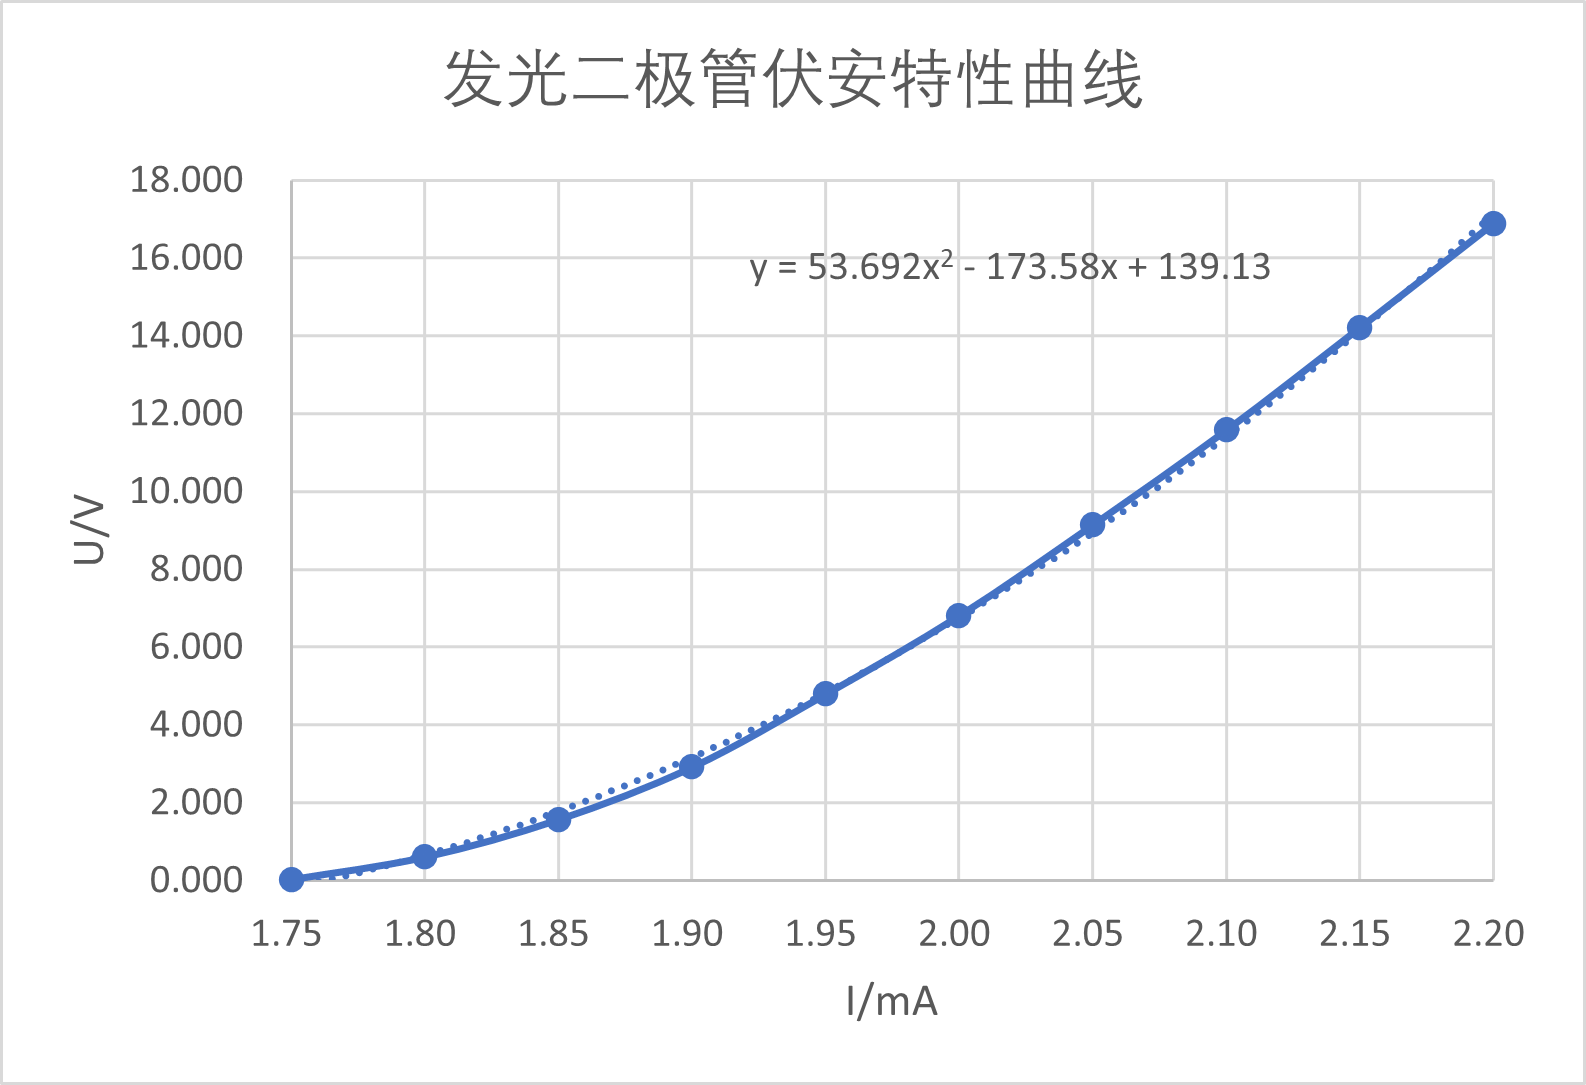
\includegraphics[width=10cm]{Fig/1.png}
            \caption{发光二极管的伏安特性曲线}
        \end{figure}
  
    \end{enumerate}
    \item 色环电阻的伏安特性曲线
    \begin{enumerate}
        \item 和上一实验过程相同。
        % Table generated by Excel2LaTeX from sheet 'Sheet1'
        \begin{table}[H]
          \centering
          \caption{色环电阻伏安特性}
          \vspace*{1em}
            \begin{tabular}{|l|r|r|r|r|r|r|r|r|r|r|r|}\hline
            U/V   & 3.0   & 2.9   & 2.8   & 2.7   & 2.6   & 2.5   & 2.4   & 2.3   & 2.2   & 2.1   & 2.0  \\\hline
            I/mA  & 2.951  & 2.853 & 2.754 & 2.656 & 2.555 & 2.456 & 2.357 & 2.258 & 2.159 & 2.061 & 1.961 \\\hline
            U/V   & 1.9   & 1.8   & 1.7   & 1.6   & 1.5   & 1.4   & 1.3   & 1.2   & 1.1   & 1.0   &  \\\hline
            I/mA  & 1.865 & 1.765 & 1.667 & 1.568 & 1.471 & 1.373 & 1.274 & 1.175 & 1.078 & 0.978 &  \\\hline
            \end{tabular}%
          %\label{tab:addlabel}%
        \end{table}%
        \begin{figure}[H]
            \centering
            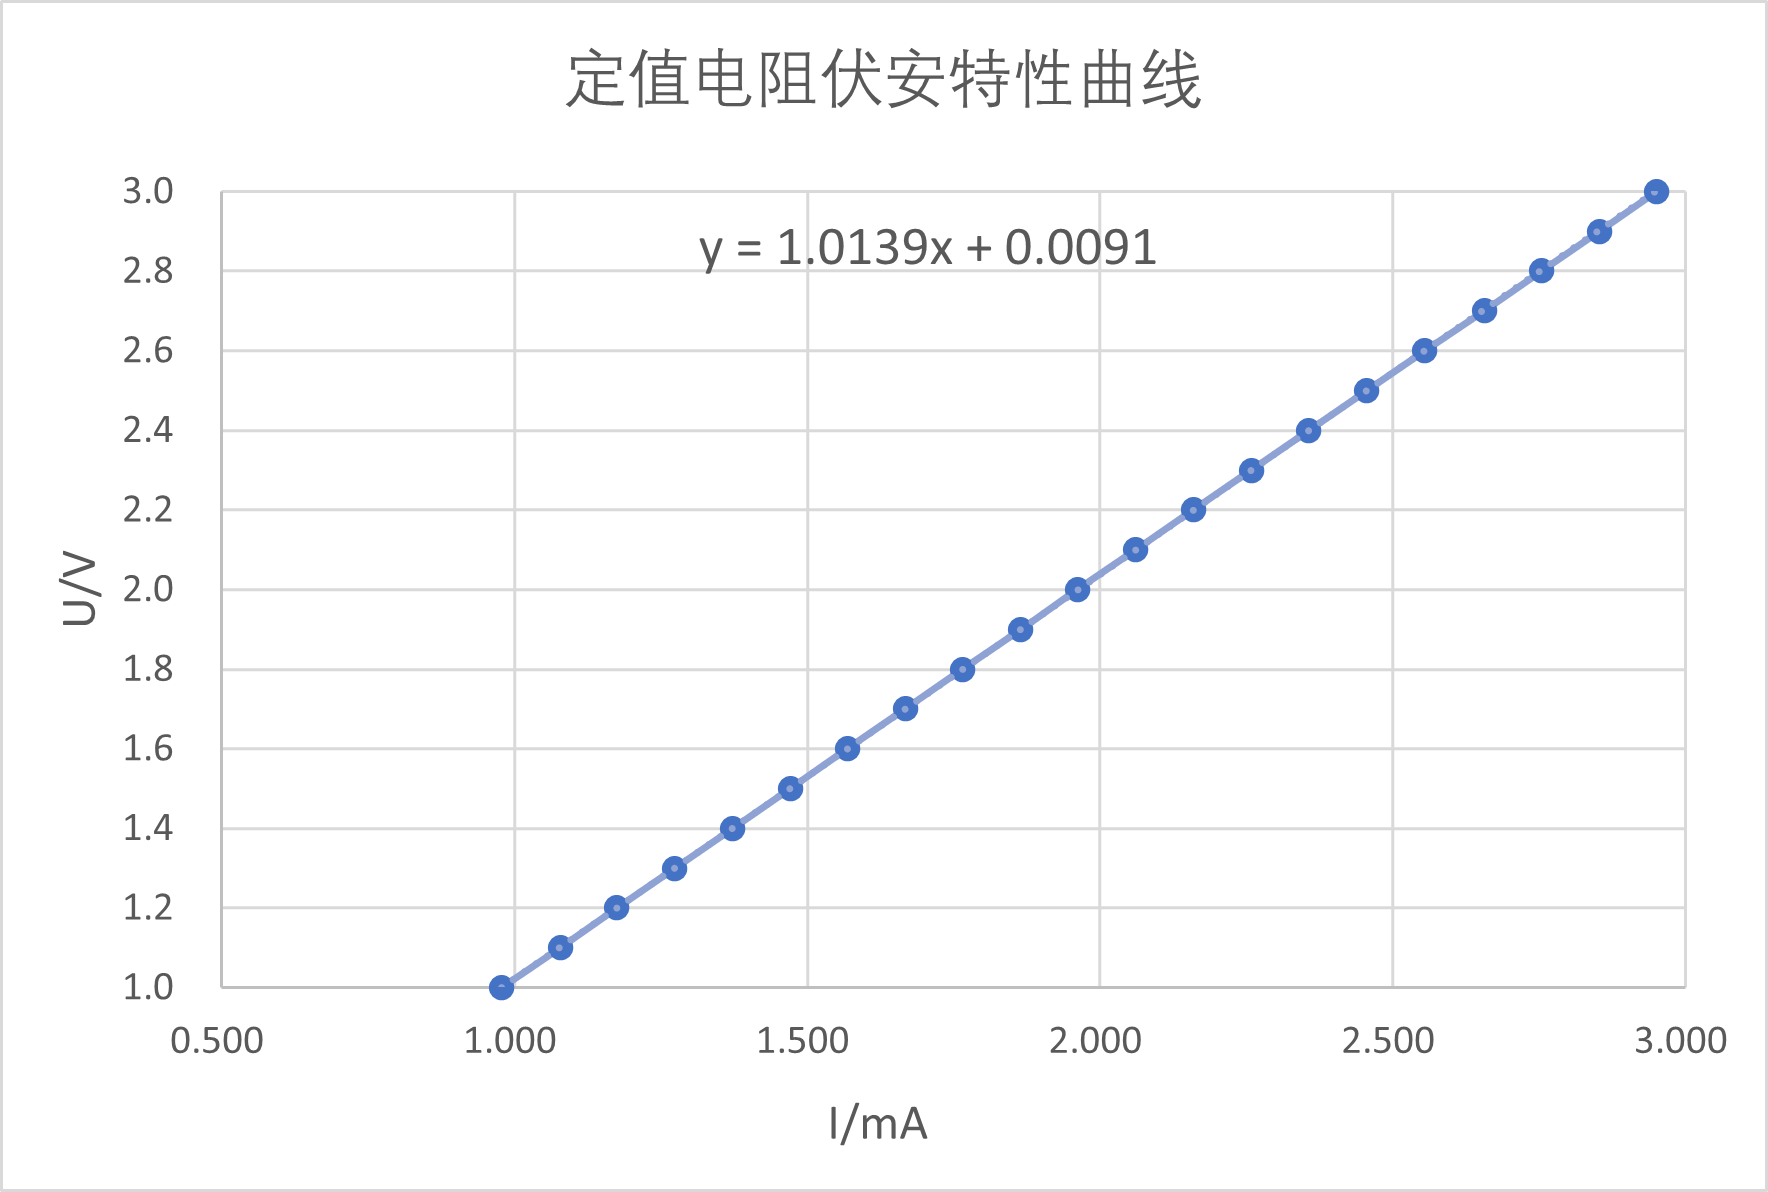
\includegraphics[width=10cm]{Fig/2.png}
            \caption{色环电阻的伏安特性曲线}
        \end{figure}
    \end{enumerate}

    \item 加入滑动变阻器后发光二极管的伏安特性曲线
    \begin{enumerate}
        \item 滑动变阻器采用限流接法接入电路。需要同时测量发光二极管的电压,电流。发光二极管电阻较小,电流表外接。
        \item 使用万用电表测量滑动变阻器的最大阻值为493.7Ω。
        % Table generated by Excel2LaTeX from sheet 'Sheet1'
        \begin{table}[H]
          \centering
          \caption{发光二极管伏安特性曲线}
          \vspace*{1em}
            \begin{tabular}{|l|r|r|r|r|r|r|r|r|r|r|r|r|}\hline
            U/V   & 1.780  & 1.785  & 1.790  & 1.795  & 1.800  & 1.805  & 1.810  & 1.815  & 1.820  & 1.830  & 1.840  & 1.850  \\\hline
            I/mA  & 0.610  & 0.695  & 0.776  & 0.865  & 0.973  & 1.091  & 1.224  & 1.366  & 1.545  & 1.888  & 2.362  & 2.948  \\\hline
            U/V   & 1.860  & 1.870  & 1.880  & 1.890  & 1.900  & 1.915  & 1.926  & 1.934  & 1.937  & 1.942  & 1.948  & 1.960  \\\hline
            I/mA  & 3.555  & 4.281  & 5.151  & 6.099  & 7.078  & 8.854  & 10.616  & 11.789  & 12.082  & 13.112  & 13.989  & 16.052  \\\hline
            \end{tabular}%
          %\label{tab:addlabel}%
        \end{table}%
        \begin{figure}[H]
            \centering
            \begin{minipage}[H]{0.49\linewidth}
                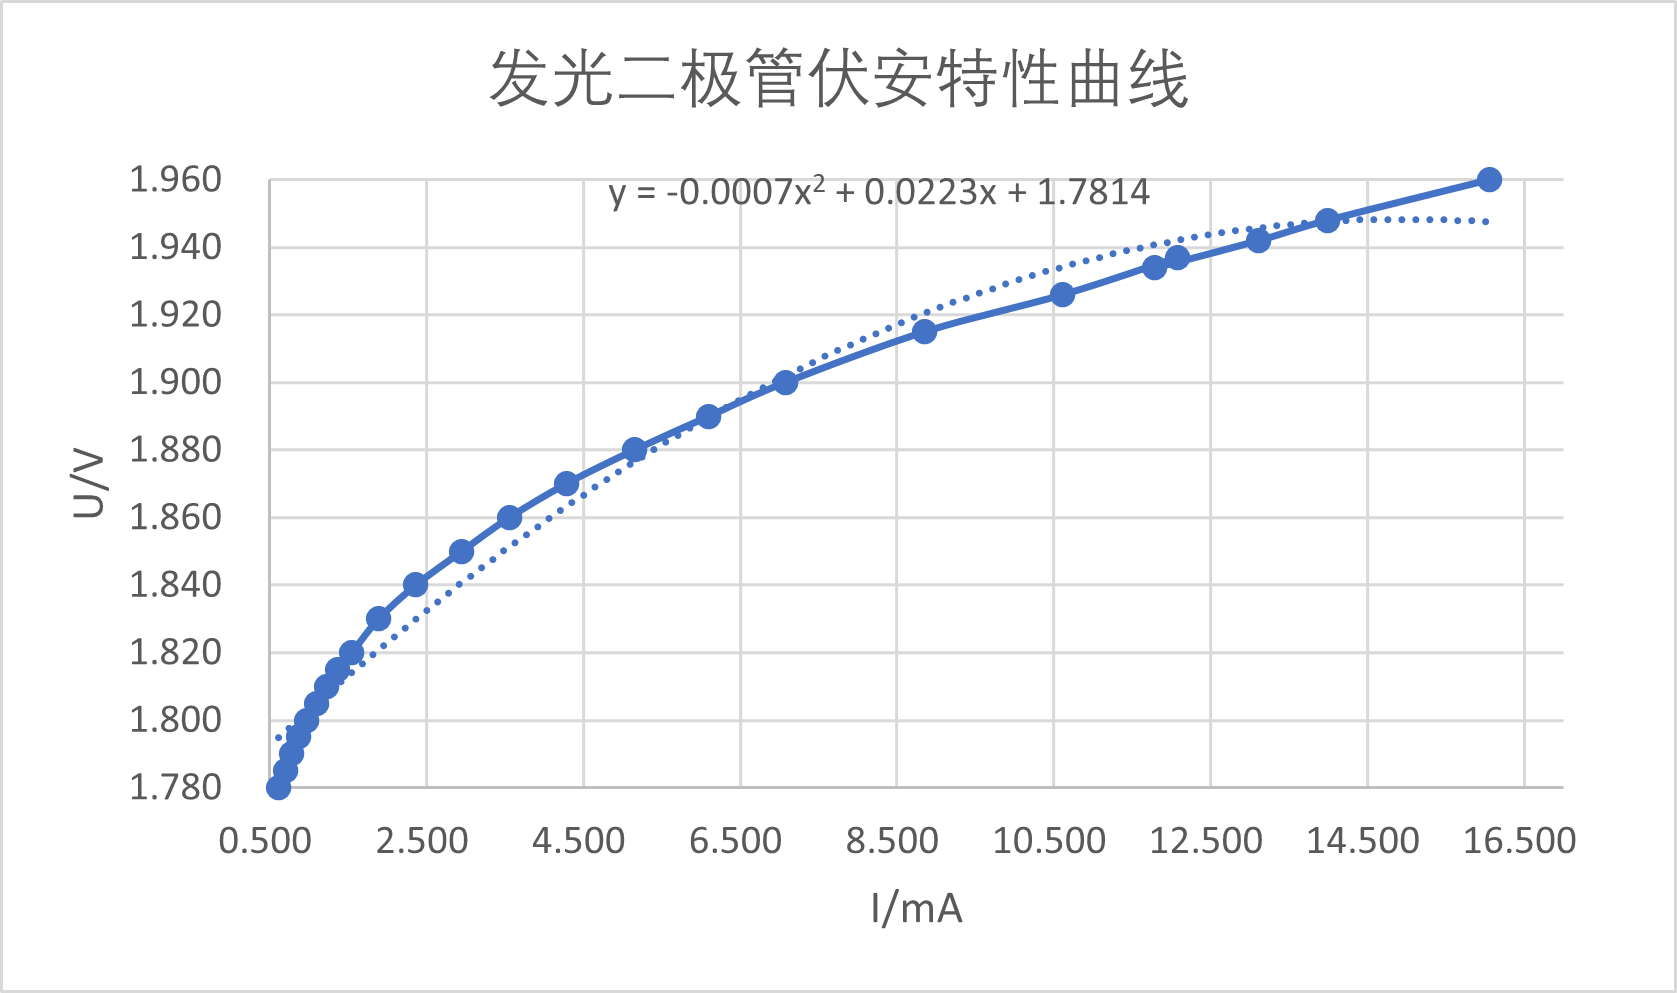
\includegraphics[width=7cm]{Fig/3.png}
                \caption{发光二极管的伏安特性曲线}
            \end{minipage}
            \begin{minipage}[H]{0.49\linewidth}
                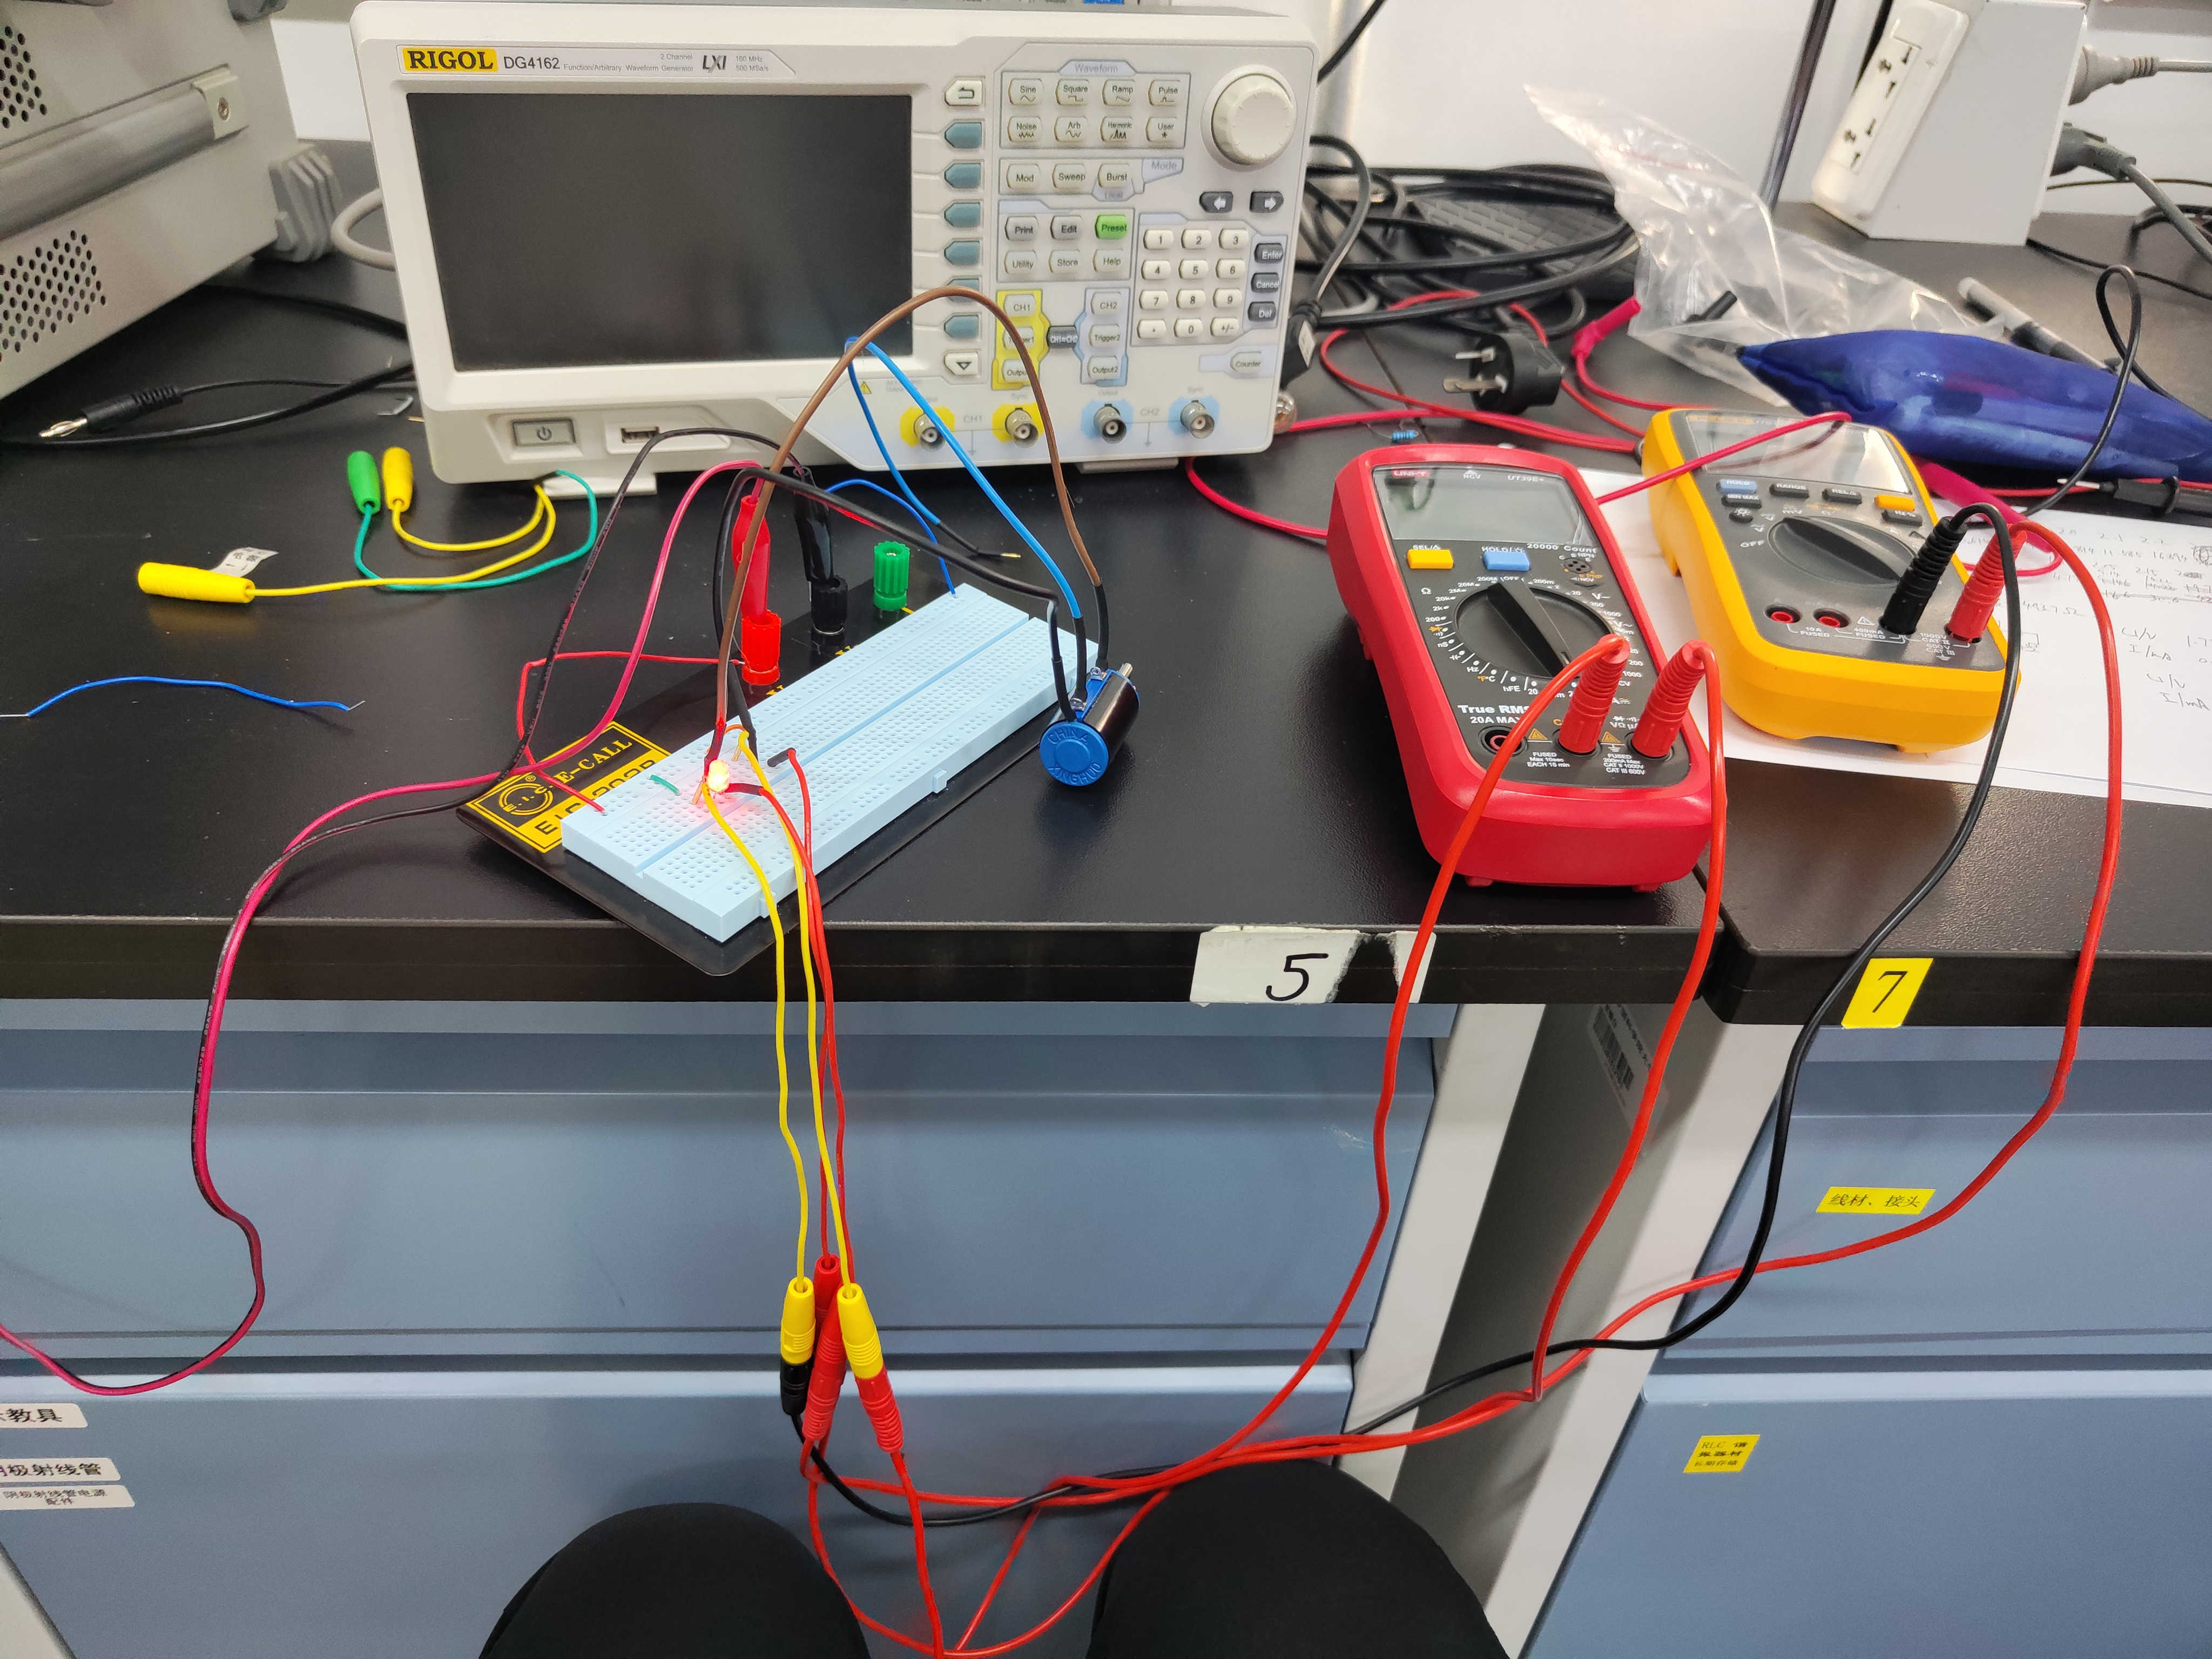
\includegraphics[width=7cm]{Fig/4.jpg}
                \caption{线路图}
            \end{minipage}
        \end{figure}
    \end{enumerate}
    \item 半波与全波整流电路
    \begin{enumerate}
        \item 半波整流电路如图,同时接入原波进行对比。
        \begin{figure}[H]
            \centering
            \begin{minipage}[H]{0.49\linewidth}
                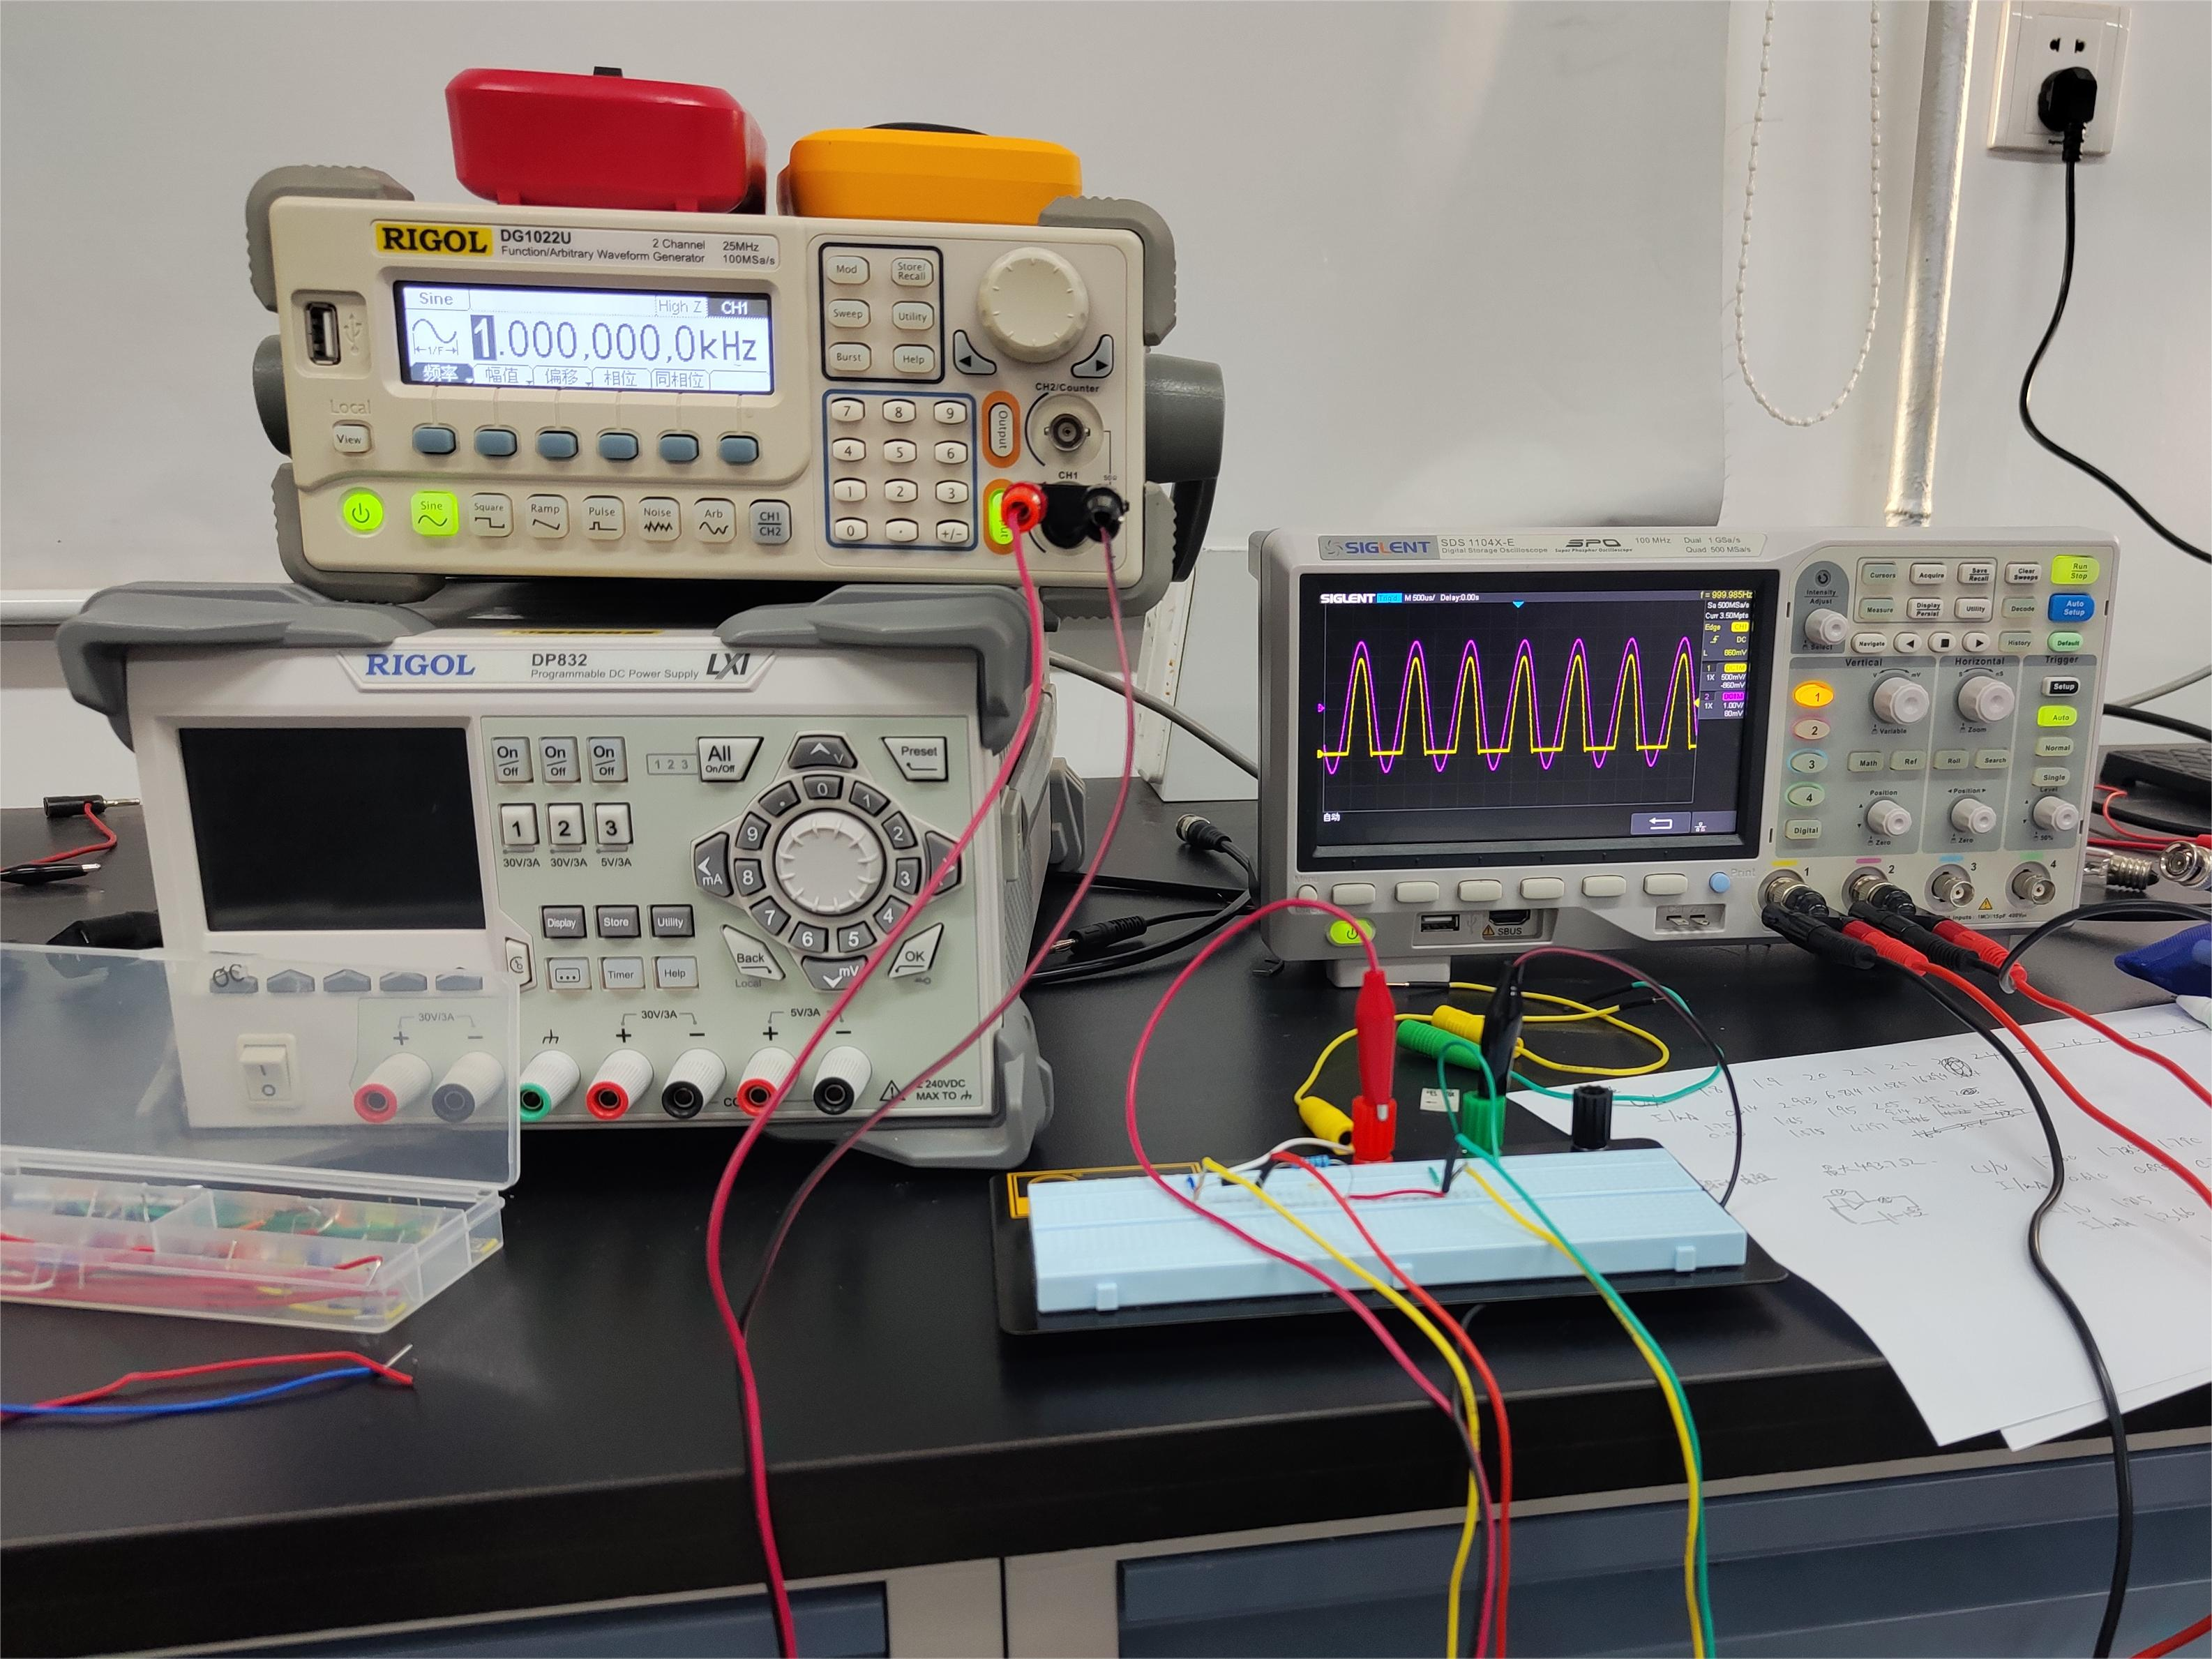
\includegraphics[width=7cm]{Fig/5.jpg}
                \caption{线路图}
            \end{minipage}
            \begin{minipage}[H]{0.49\linewidth}
                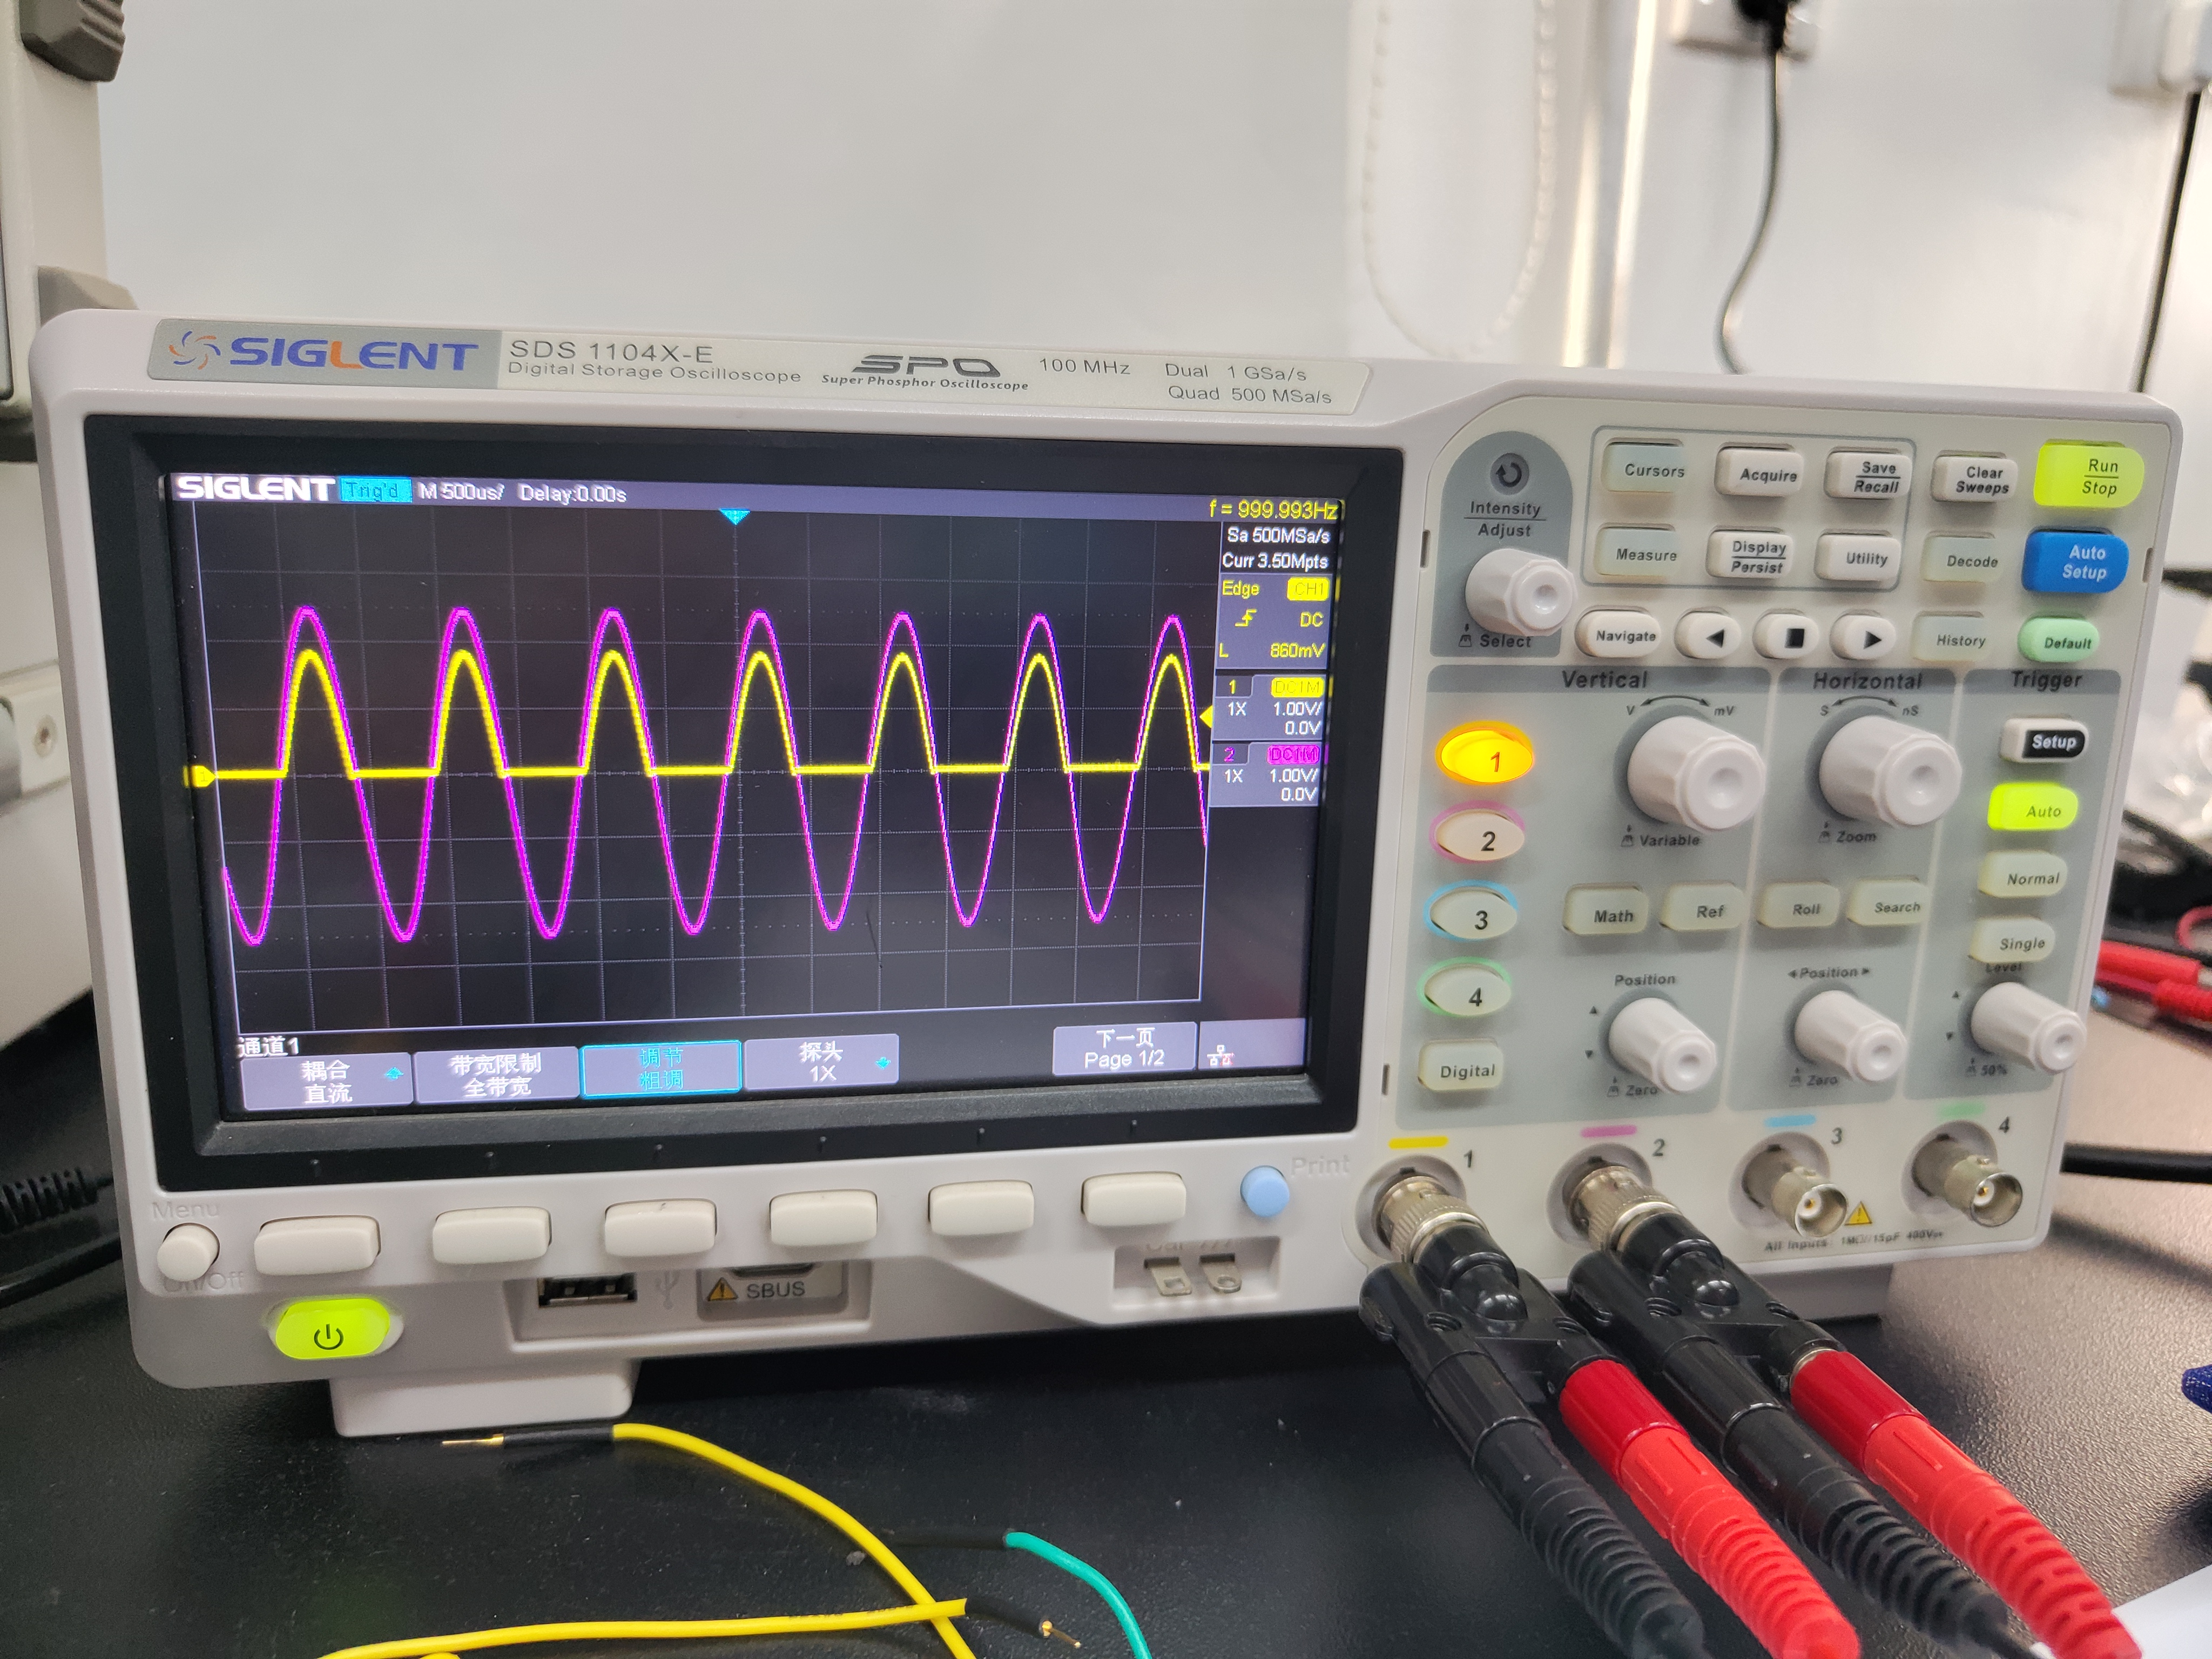
\includegraphics[width=7cm]{Fig/6.jpg}
                \caption{半波与原波}
            \end{minipage}
        \end{figure}
        \item 全波整流电路如图,采用PN结方式接入,同时使用math计算合成两个半波生成全波。
        \begin{figure}[H]
            \centering
            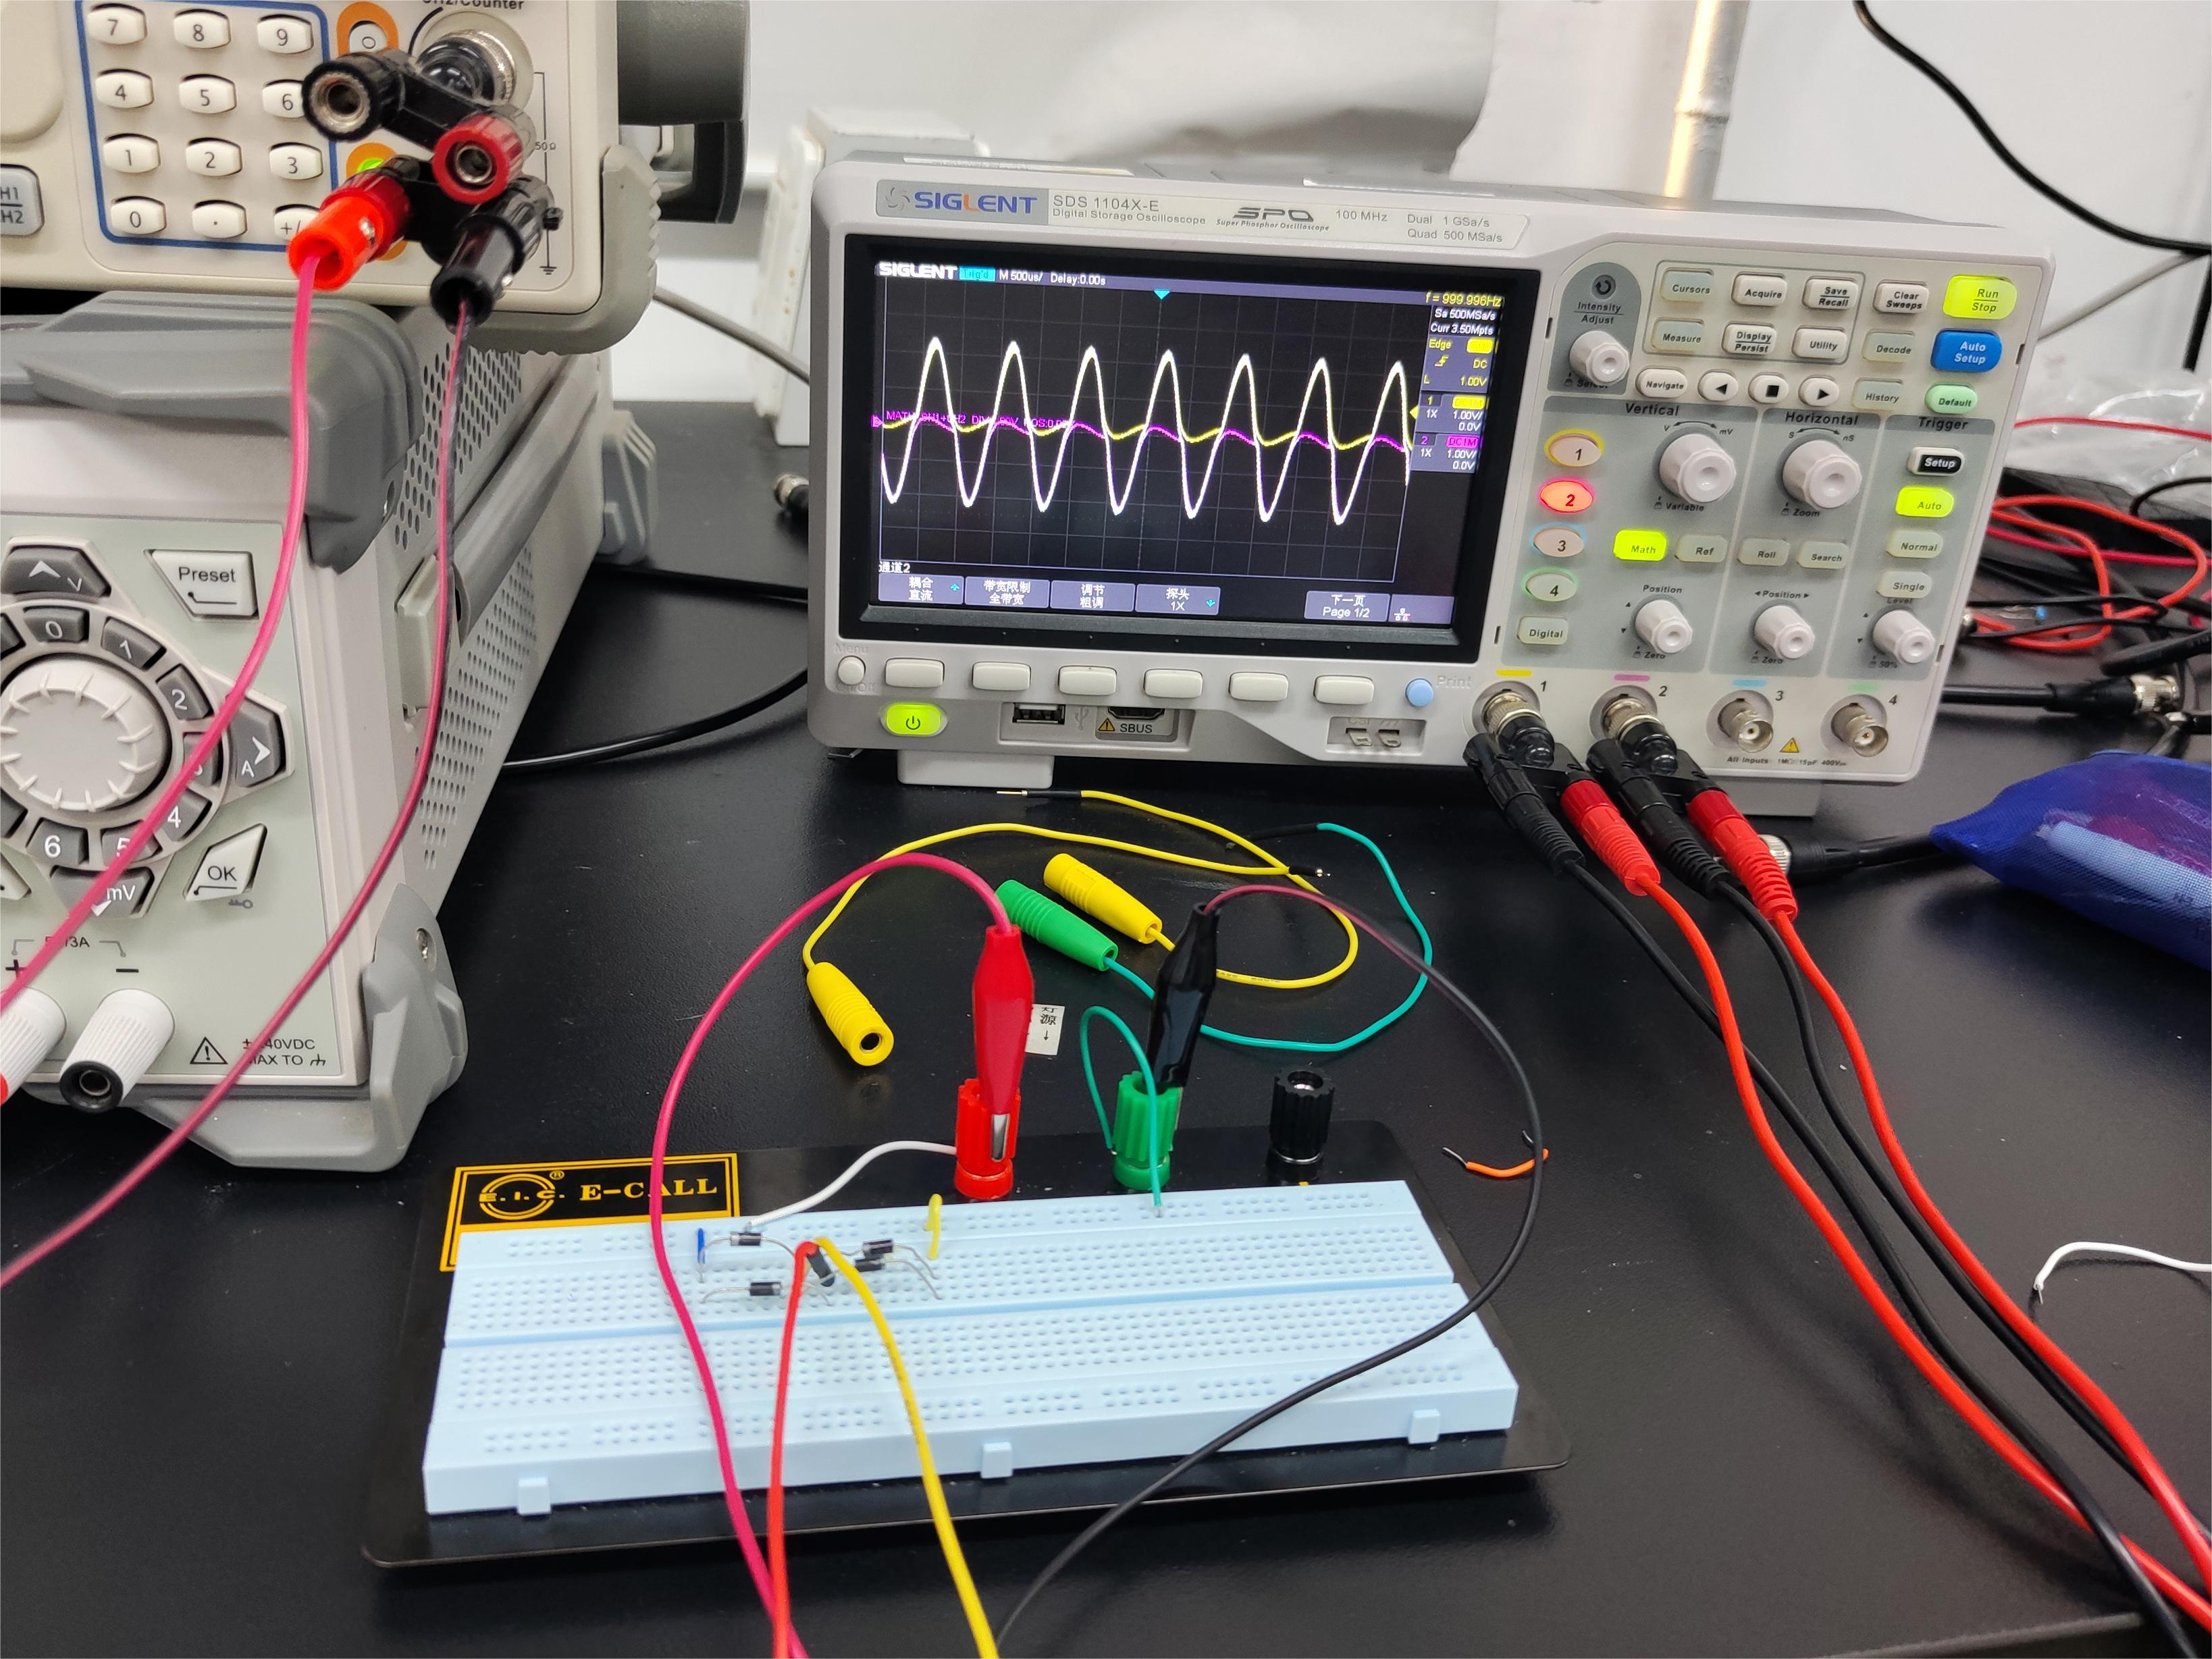
\includegraphics[width=10cm]{Fig/7.jpg}
            \caption{全波整流与电路图}
        \end{figure}
    \end{enumerate}
\end{enumerate}

\section{实验反思、收获与总结}
\begin{enumerate}
    \item 接入滑动变阻器之前一定要确认其阻值范围。
    \item 全波整流电路较难实现,可以采用PN结或者双输出的方式。
\end{enumerate}


\begin{center}
    \vspace*{1em}
    \Large \bf 第二部分\qquad 实验原始记录
\end{center}
\begin{figure}[H]
    \centering
    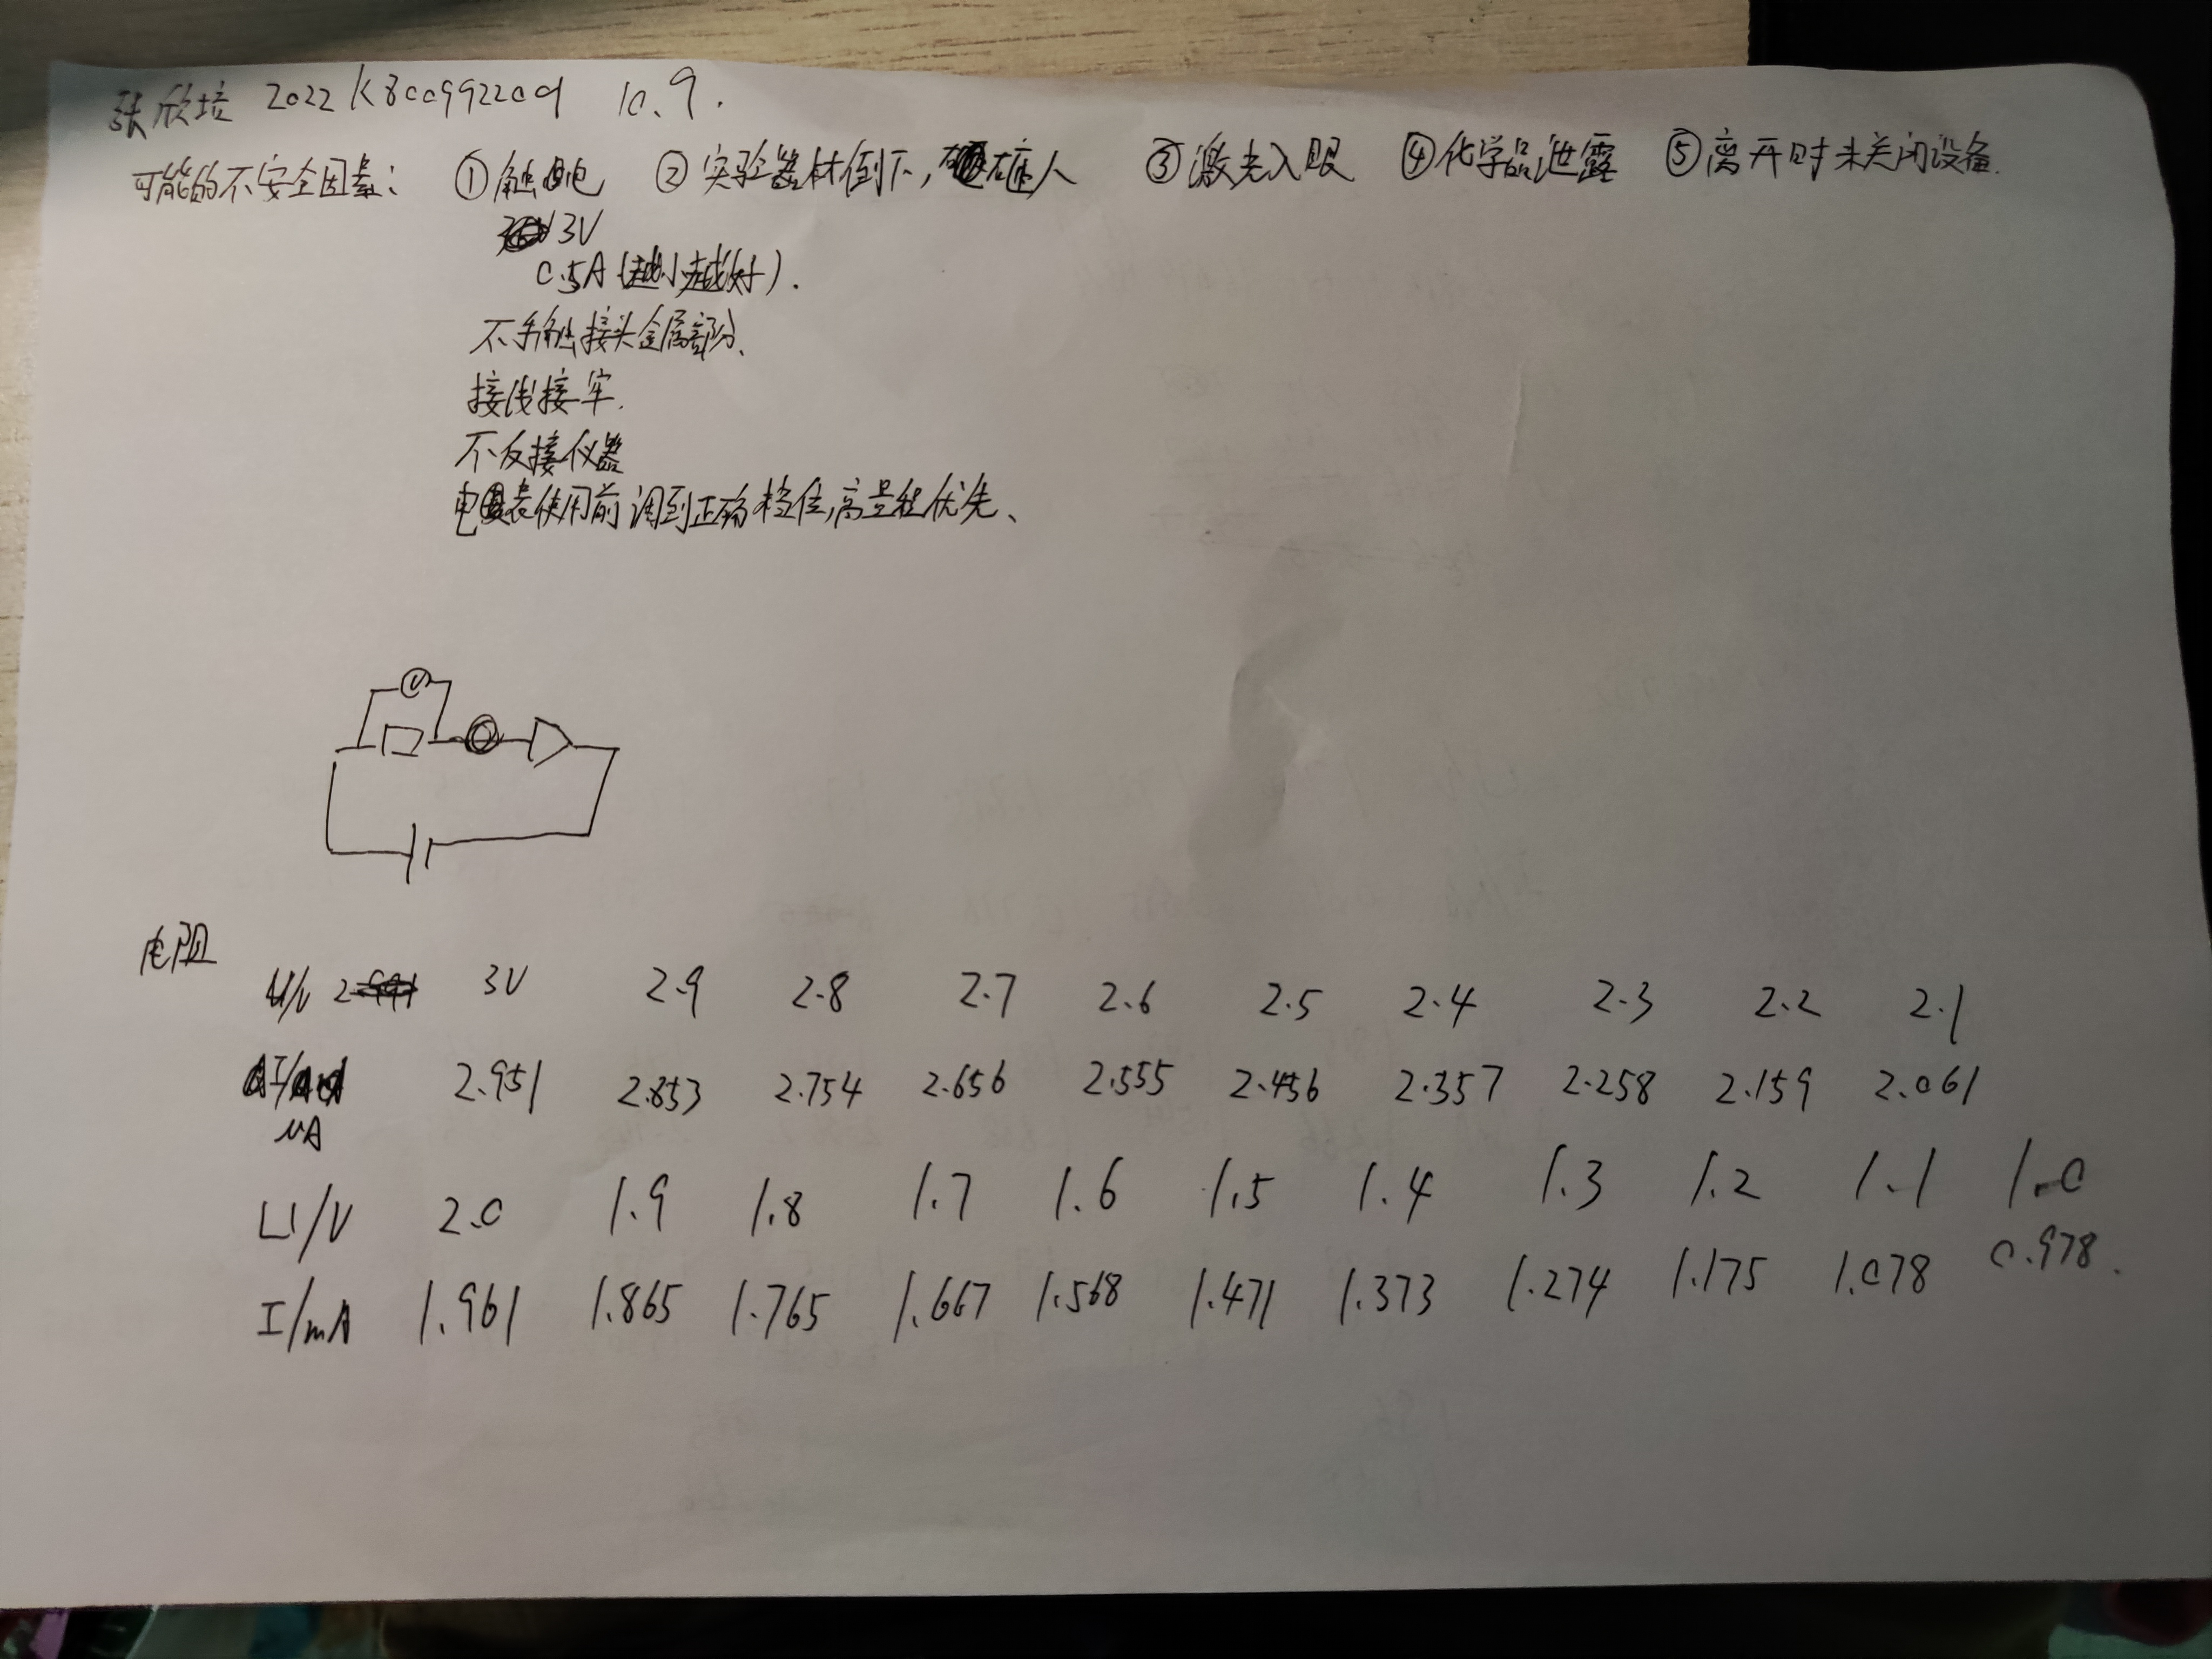
\includegraphics[width=15cm]{Fig/8.jpg}
    \caption{实验记录1}
    \vspace*{1em}
    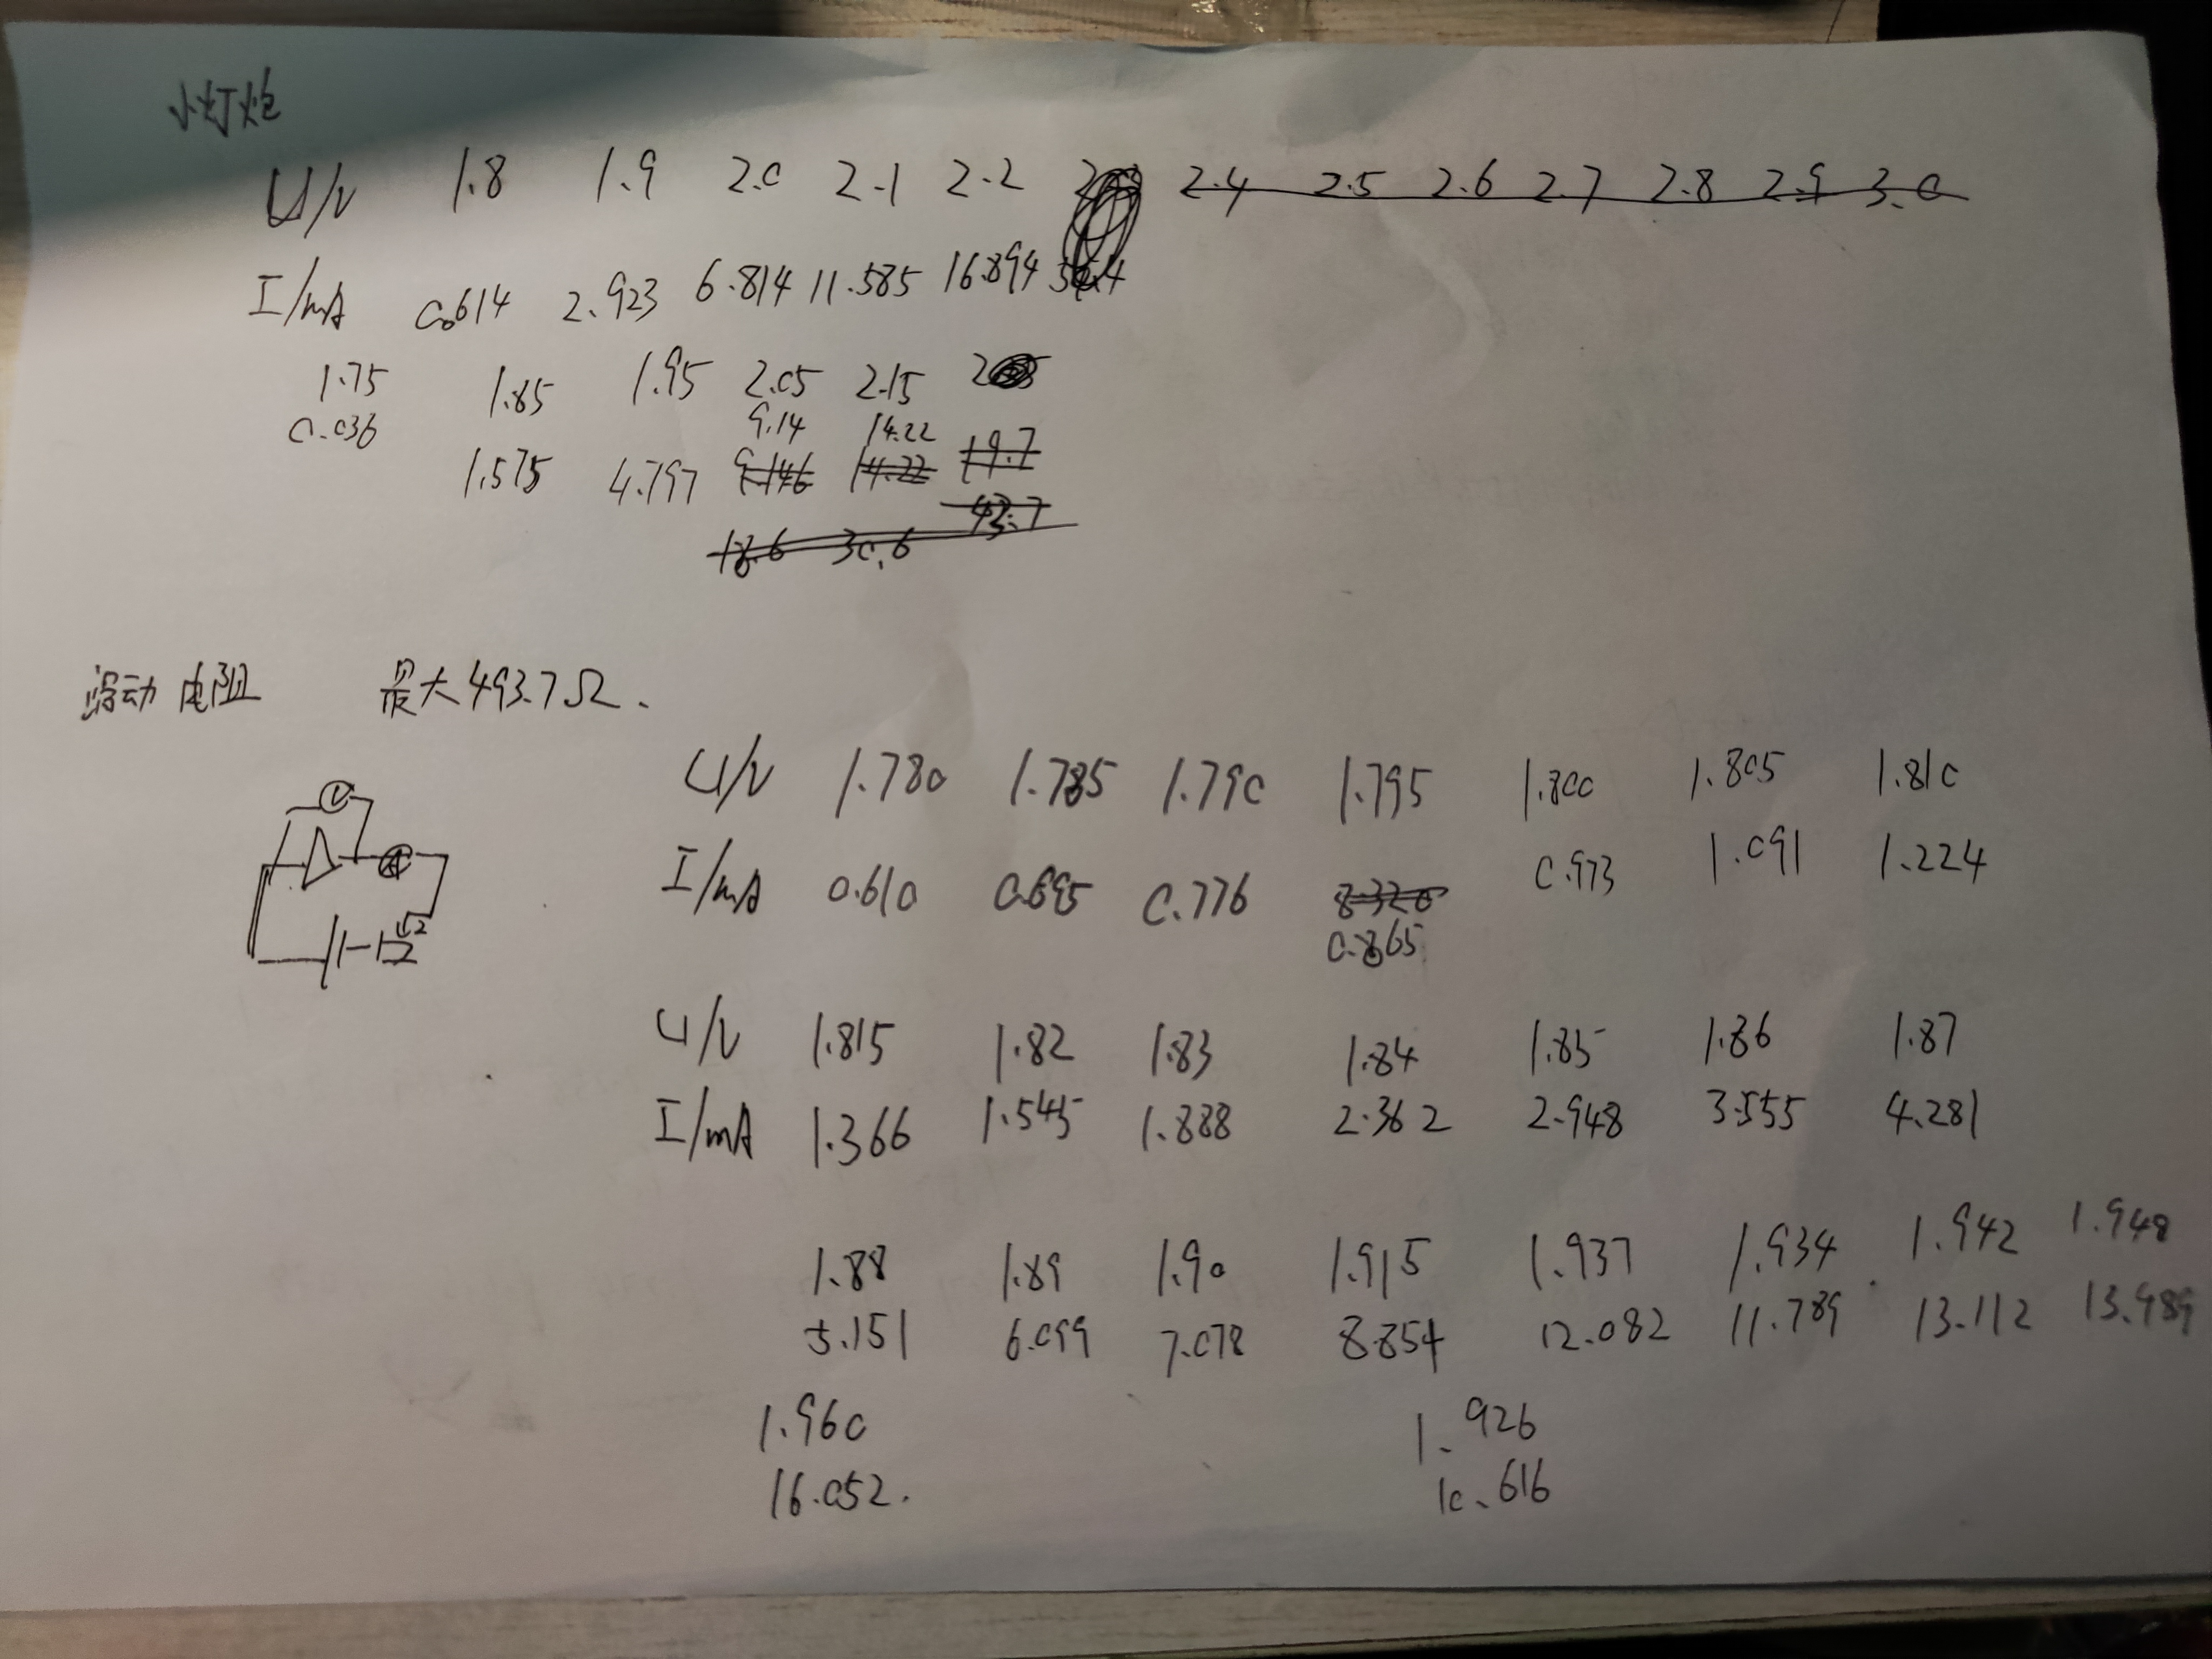
\includegraphics[width=15cm]{Fig/9.jpg}
    \caption{实验记录2}
\end{figure}



\end{document}